\documentclass[12pt]{article}
\usepackage{graphicx}
\usepackage{amsmath}
\usepackage{listings}
\usepackage{hyperref}
\usepackage{colortbl}
\usepackage{array}
\usepackage{tabularx}
\usepackage{caption}
\usepackage[a4paper, margin=1in]{geometry}
\usepackage{parskip}
\usepackage{titlesec}
\usepackage{xcolor}

\titleformat{\section}[block]{\normalfont\Large\bfseries\color{darkblue}}{\thesection}{1em}{}

\definecolor{lightgray}{gray}{0.9} 
\definecolor{darkblue}{rgb}{0.0, 0.2, 0.6}


\title{MailGPT: A GPT-Integrated Email Service for Dynamic Content Generation}
\author{
    Yosep Kim\textsuperscript{1}, 
    Dohyun Bu\textsuperscript{2}, 
    Sumin Lim\textsuperscript{3}, 
    Miseo Joung\textsuperscript{4}, 
}
\date{\today}

\begin{document}
\maketitle

\begin{center}
	\textsuperscript{1,2,3,4}Sungkyunkwan University\\
	\href{https://mailgpt.intueri.cloud}{https://mailgpt.intueri.cloud}
\end{center}
\begin{abstract}
	In the digital communication era, email remains a pivotal tool for professional interactions. Despite its prevalence, composing a proficient email that encapsulates clarity, conciseness, and the appropriate tone can be complex. Miscommunications in such contexts can inadvertently lead to undesired consequences. MailGPT introduces a novel solution by integrating the GPT API to facilitate dynamic email content creation suited to user intent. This system is technologically underpinned by React for frontend design, Docker for deployment, and SQLite for data management, establishing it as a potential game-changer in digital communication. Its architecture is modular, ensuring adaptability, and incorporates a user-friendly workflow. With the collaborative expertise of team members like Yosep Kim, Dohyun Bu, Sumin Lim, and Miseo Joung, MailGPT seeks to redefine the realm of email drafting.
\end{abstract}
\section{Introduction}

In the current digital age, email remains a primary medium for professional communication. Yet, for many, crafting an effective email—balancing clarity, conciseness, and the desired tone—can be a daunting task. The challenges of email writing are compounded when one has to ensure consistency and professionalism across myriad scenarios, from addressing a superior or a client to communicating with a colleague. 

\subsection{Motivation}

The essence of these challenges stems from the inability of individuals to quickly adapt their writing styles to different contexts. A miscommunication or a misinterpreted tone can have unintended consequences, affecting relationships and business outcomes. Therefore, it's imperative to strike the right balance, ensuring that the content of the email aligns perfectly with its intent.

\subsection{Solution: MailGPT}

Enter MailGPT: a revolutionary approach to email writing. This service integrates the powerful language capabilities of the GPT API, offering dynamic email content generation tailored to the user's requirements. By simply specifying the target and mood of the email, users are provided with content that matches their intent, eliminating the common pain points of email drafting.

\subsection{Technical Backbone}

Underpinning MailGPT is a robust technological framework. It leverages the capabilities of React for frontend development, ensuring a responsive and intuitive user interface. Docker facilitates easy deployment, ensuring that the application remains scalable and resilient. The data backbone of the application, including email drafts and user preferences, is managed through SQLite, a versatile and efficient database solution. The fusion of these technologies, coupled with the intelligence of the GPT API, positions MailGPT as a forerunner in transforming digital communication.


\section{System Architecture}

The system architecture of our application is robust and designed to handle the modern demands of real-time processing. Built on a modular structure, it offers scalability, maintainability, and ease of enhancements.

\subsection{Components}
Our system is divided into three core components, each dedicated to performing its task efficiently:
\begin{itemize}
	\item \textbf{Frontend}: Developed using React, a popular React framework known for its server-side rendering capabilities. It ensures a seamless user experience, catering to a responsive design that is adaptable across devices of varying sizes.
	      	          
	\item \textbf{Backend}: Developed using Fast API, a high-performance framework for building web applications. This component is responsible for the system's core logic, including its interaction with SQLite and the GPT API. It plays a pivotal role in data processing and content generation.
	      	          
	\item \textbf{Database}: We've opted for SQLite as our primary data store. 
\end{itemize}

\subsection{Workflow}
The workflow is straightforward and user-centric. Upon accessing the platform, users are prompted to provide the target email and their desired mood or tone for the email content. This leads to a sequence of operations:

The frontend, harnessing the capabilities of React, utilizes a predefined template to generate a unique prompt based on the user's input. This prompt is securely stored in SQLite for future reference. Following this, the backend, powered by Fast API, dispatches the prompt to the GPT API. The GPT API, using its advanced natural language processing capabilities, crafts an appropriate email content tailored to the user's requirements. This content is returned in Markdown format, allowing users to view a well-structured preview.

If the user is satisfied with the generated content, a confirmation is obtained. Subsequently, the content is sent to the designated target email address using SMTP, ensuring timely and reliable delivery.

\section{Technical Details}

\subsection{Frontend}
The frontend, developed using the sophisticated React framework, serves as the gateway to our application. It's the first point of contact for users, offering them an intuitive interface to input their requirements. Built with a responsive design, it ensures accessibility across a myriad of devices, from desktops to smartphones. It is designed to be both visually appealing and functional, enhancing user engagement and satisfaction.

\subsection{Backend}
At the heart of our application lies the backend, which orchestrates a symphony of operations:

\begin{enumerate}
	\item \textbf{Interaction with SQLite}: Even though SQLite serves as our primary database, we leverage SQLite for certain relational data requirements. It provides a robust and efficient platform for data storage and retrieval.
	      	          
	\item \textbf{Sending the prompt to the GPT API}: The core functionality. Based on user inputs, the system creates a custom prompt. This is dispatched to the GPT API, awaiting its magic of content generation.
	      	          
	\item \textbf{Receiving and returning the generated content to the frontend}: Once the GPT API generates the content, it's the backend's responsibility to receive it, process it if needed, and relay it to the frontend. This ensures that users receive a swift response, enhancing their overall experience.
\end{enumerate}

\subsection{Data Flow Diagrams}

The intricate interplay between the frontend and backend of MailGPT is aptly captured using detailed data flow diagrams. These diagrams, while complex in their representation, serve as a beacon for understanding the delicate choreography of data exchange and processing that ensues within our system. The multifarious activities and communication pathways, showcasing the convergence of various system modules, are intricately laid out in these diagrams. 

Our decision to utilize such expressive visuals stems from the quintessential need for clear and precise elucidation of the interactions between different system components. For developers, stakeholders, and even advanced users, these diagrams provide invaluable insights into the internal workings of our platform. They unravel the layered intricacies and underscore the robustness of our application’s design.

Furthermore, while the user interface presents a polished and seamless experience to the end-users, it's the underlying data flows and transactions, meticulously visualized in our diagrams, that fortify the application's reliability and performance. Hence, these diagrams become an instrumental tool, not just for design and development, but also for troubleshooting, optimization, and further enhancements to our cutting-edge platform.


\subsubsection{GPT API Data Flow}

As depicted in Figure \ref{fig:gpt_api_flow}, the GPT API data flow underpins MailGPT's operation, demonstrating a meticulously orchestrated interaction among various components.

Upon a user's request, the system channels the call from the client terminal to our EC2 instance, initially interfacing with the Nginx for efficient load balancing. The request subsequently traverses the React framework for preliminary processing and then to FastAPI, an ASGI framework ensuring rapid processing and data integrity. At the crux of this sequence, the GPT API server, fortified with advanced algorithms, processes and contextualizes the request, transforming it into coherent outputs.

The processed data, rich with insights, retraces its steps, passing through FastAPI and React for final optimization before Nginx ensures its prompt return to the user. This streamlined flow epitomizes efficiency and reliability in MailGPT's infrastructure.


\begin{figure}[ht]
	\centering
	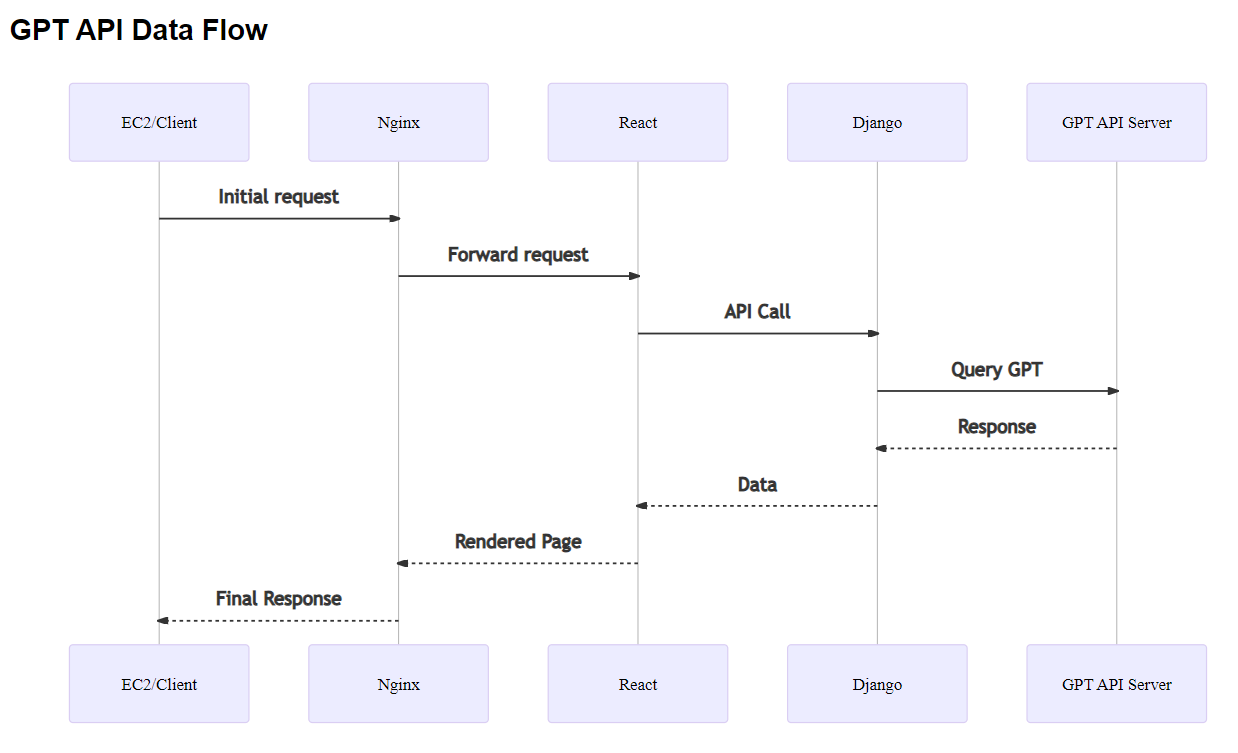
\includegraphics[width=0.8\textwidth]{gpt_api_flow.png}
	\caption{Data flow diagram illustrating the GPT API communication process}
	\label{fig:gpt_api_flow}
\end{figure}

\subsubsection{smtplib Data Flow}

The symphony of our email notification system finds its muse in the data flow depicted in Figure \ref{fig:smtplib_flow}. Like a familiar tune, the journey originates with the client's sincere request. This beacon of communication is then acknowledged by the frontend, initiating a series of orchestrated movements. The backend, acting as the maestro, liaises with the email server, crafting a melodious email notification. As the server resonates with the acknowledgment of successful dispatch, the backend, not missing a beat, alerts the frontend. The finale witnesses the frontend conveying this melodious success back to the awaiting client.

\begin{figure}[ht]
	\centering
	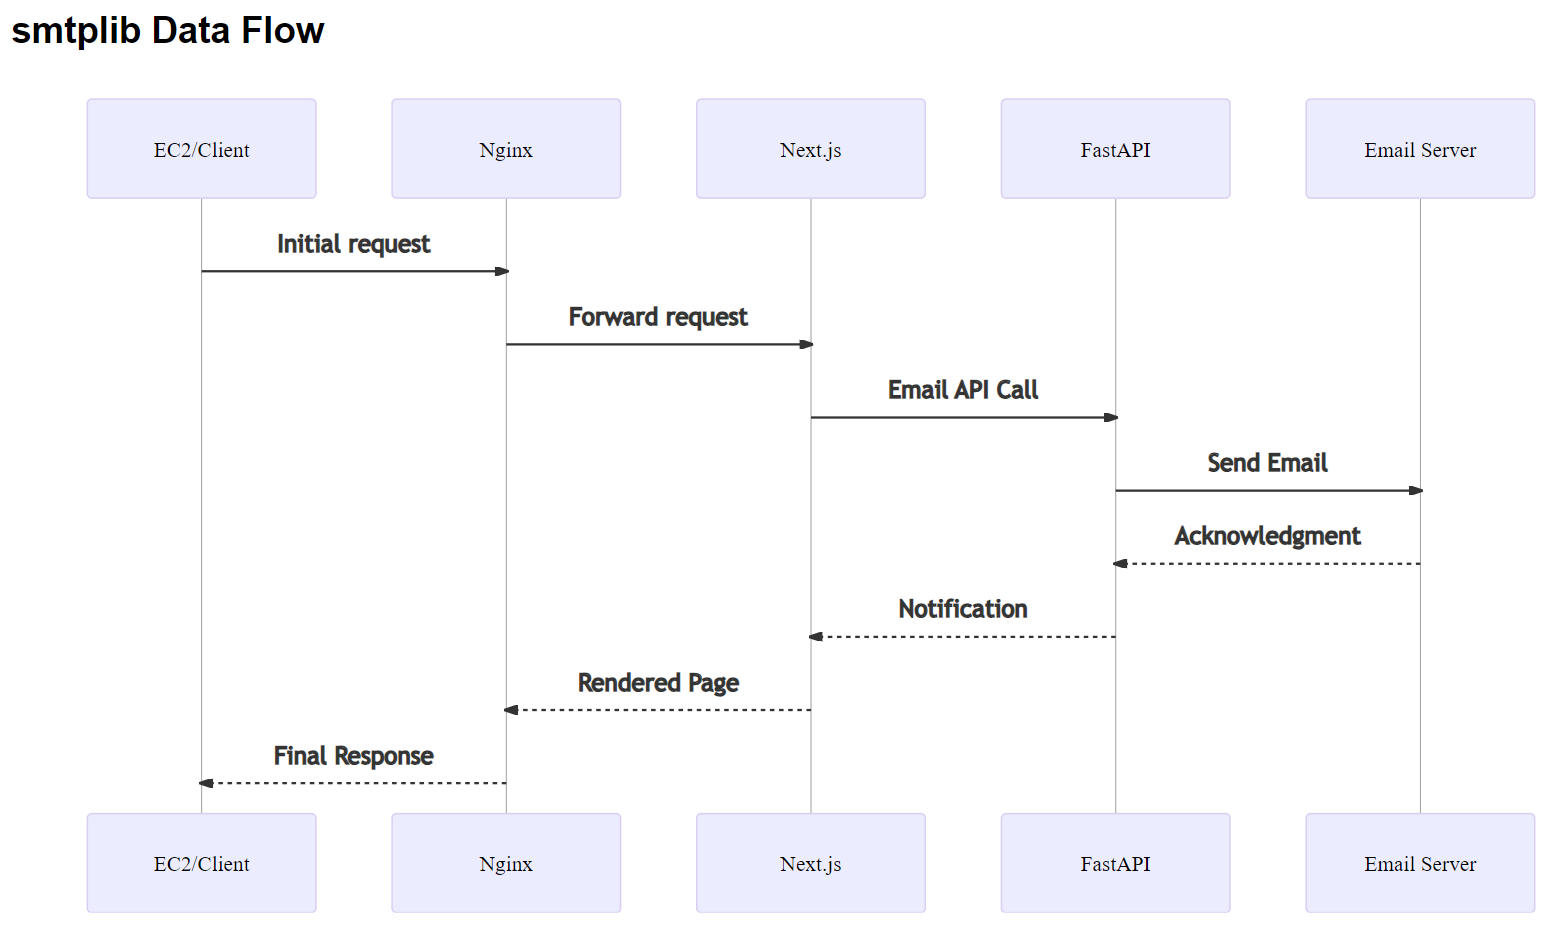
\includegraphics[width=0.8\textwidth]{smtplib_flow.png}
	\caption{Data flow diagram illustrating the smtplib communication process}
	\label{fig:smtplib_flow}
\end{figure}

\subsection{Conclusion}

Our platform's technical tapestry is woven with precision, where every thread represents a service or technology that contributes to the grand design. By employing avant-garde tools and technologies and ensuring a harmonious flow of data, we present to our users a masterpiece of efficiency and reliability. From the warm embrace of the frontend to the rhythmic cadence of the backend, every facet of our application has been chiseled to perfection, promising an experience that is both memorable and unparalleled.


\subsection{Detailed Database Design}

Our database comprises three core tables: \textit{LOGIN}, \textit{HISTORY}, and \textit{SETTINGS}. Their inter-relationships and attributes are illustrated in the ER Diagram (Figure \ref{fig:er_diagram}). 

\begin{figure}[ht]
	\centering
	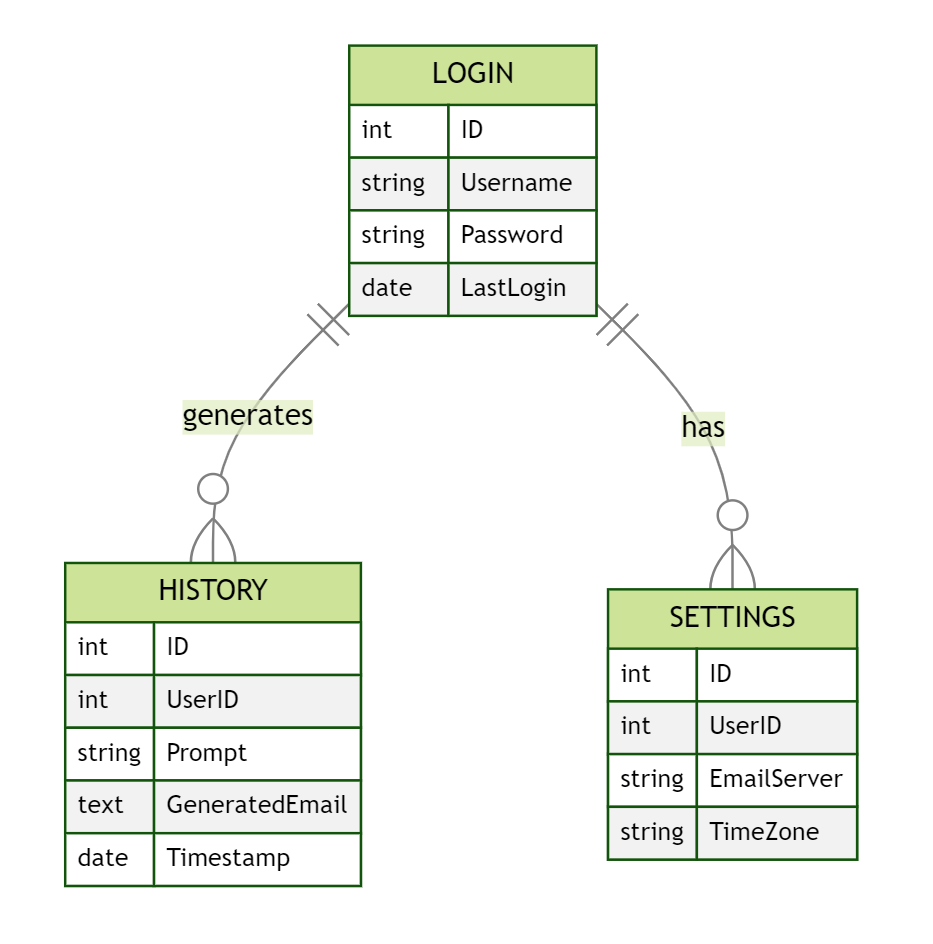
\includegraphics[width=0.8\textwidth]{ER_Diagram.png}
	\caption{Entity-Relationship Diagram for the MailGPT Database}
	\label{fig:er_diagram}
\end{figure}

\subsubsection{LOGIN Table}
The \textit{LOGIN} table stores user login details. Key attributes include:
\begin{itemize}
	\item \textbf{ID:} A unique identifier for each user.
	\item \textbf{Username:} The login name used by the user.
	\item \textbf{Password:} The encrypted password.
	\item \textbf{LastLogin:} Timestamp of the user's last login.
\end{itemize}

\subsubsection{HISTORY Table}
The \textit{HISTORY} table keeps a record of all email prompts and the generated content based on them. Key attributes include:
\begin{itemize}
	\item \textbf{ID:} A unique identifier for each record.
	\item \textbf{UserID:} Foreign key relating back to the \textit{LOGIN} table.
	\item \textbf{Prompt:} The initial email prompt provided by the user.
	\item \textbf{GeneratedEmail:} The content produced by the GPT API.
	\item \textbf{Timestamp:} The exact time the email content was generated.
\end{itemize}

\subsubsection{SETTINGS Table}
The \textit{SETTINGS} table holds configuration data for each user. Key attributes include:
\begin{itemize}
	\item \textbf{ID:} A unique identifier for each settings record.
	\item \textbf{UserID:} Foreign key relating back to the \textit{LOGIN} table.
	\item \textbf{EmailServer:} The user's email server details.
	\item \textbf{TimeZone:} The user's preferred timezone.
\end{itemize}

The relationships indicate that a user in the \textit{LOGIN} table can have multiple entries in both the \textit{HISTORY} and \textit{SETTINGS} tables. This signifies that each user can generate multiple email contents and have multiple settings configurations.

\section{Role and Time Line}

\subsection{Time Line}

The Agile Scrum methodology's Gantt chart showcases the progression of the project over three sprints, spanning three months. Tasks are divided among these sprints to ensure efficient and timely completion.

\begin{table}[ht]
	\centering
	\begin{tabularx}{\textwidth}{|X|c|c|c|}
		\hline
		\rowcolor{gray!30}
		Task                         & Sprint 1       & Sprint 2        & Sprint 3       \\
		\hline
		\rowcolor{gray!30}
				
		Time                         & Oct 1 - Oct 20 & Oct 21 - Nov 10 & Nov 11 - Dec 1 \\
		\hline
		Frontend Base Setup          & X              &                 &                \\
		\hline
		Backend DB and API Setup     & X              &                 &                \\
		\hline
		Set Project Milestones       & X              &                 &                \\
		\hline
		Frontend-Backend Integration &                & X               &                \\
		\hline
		Backend Advanced Features    &                & X               &                \\
		\hline
		Re-evaluate Milestones       &                & X               &                \\
		\hline
		Finalize UI/UX               &                &                 & X              \\
		\hline
		Backend Deployment           &                &                 & X              \\
		\hline
		Project Closure              &                &                 & X              \\
		\hline
	\end{tabularx}
	\caption{Gantt Chart for Agile Scrum Project Timeline}
\end{table}

\subsection{Team Roles}

In the journey of creating the MailGPT application, a team of adept professionals was assembled, each with specific roles and responsibilities. The table below delineates the key team members and their associated tasks:

\begin{table}[ht]
	\centering
	\begin{tabularx}{\textwidth}{|X|X|}
		\hline
		\rowcolor{gray!30}
		Team Member & Role                                                                \\
		\hline
		Yosep Kim   & Project Manager, Documentation, Backend (Cloud Infra), AI algorithm \\
		\hline
		Sumin Lim   & Frontend (React, UX/UI)                                           \\
		\hline
		Dohyun Bu & Backend (Fast API, GPT, DB), AI algorithm                           \\
		\hline
		Miseo Joung & Frontend (React, UX/UI)                                           \\
		\hline
	\end{tabularx}
	\caption{Roles and Responsibilities of the Team Members}
\end{table}

Yosep Kim leads the project, overseeing management, backend infrastructure, and AI advancements. Dohyun Bu handles backend tasks, including APIs and AI. Sumin Lim manages the frontend using React and contributes to the backend. Miseo Joung specializes in UX/UI and backend APIs. Their combined expertise drives the MailGPT project.

\titleformat{\section}[block]{\normalfont\Large\bfseries\color{darkblue}}{\thesection}{1em}{}

\section*{Conclusion}

In the age of rapid digital communication, the efficiency and clarity of our electronic correspondences play a pivotal role in both professional and personal settings. \textbf{MailGPT}'s integration with the GPT API promises a transformative approach to email composition.

The traditional method of email writing often involves considerable time and cognitive effort. This can lead to unnecessary delays, potential misunderstandings, or even missed opportunities. By intelligently generating content based on user prompts, \textbf{MailGPT} not only simplifies this process but also offers a consistently high-quality output.

Moreover, as the GPT API continues to evolve and improve, the potential for \textbf{MailGPT}'s features will only grow. There's a possibility for broader applications such as customizing email styles based on recipient preferences, generating summaries of long emails for quick reading, and even predicting user intent to further streamline the email drafting process.

Additionally, for non-native speakers or those less confident in their writing abilities, \textbf{MailGPT} can act as an invaluable tool, ensuring clarity and coherence in their emails. This democratizes the process, allowing more individuals to communicate effectively, regardless of their writing expertise.

In conclusion, \textbf{MailGPT}'s innovative approach, driven by the power of the GPT API, promises not just an evolution in email composition, but a potential revolution in digital communication as a whole. As the digital age progresses, tools like \textbf{MailGPT} will become indispensable in bridging gaps, enhancing efficiency, and making sure that communication remains at the heart of all our interactions.


\begin{thebibliography}{99}
		
	\bibitem{silberschatz} 
	A. Silberschatz, H. F. Korth, and S. Sudarshan, 
	\textit{Database system concepts}.
		
	\bibitem{chacon} 
	S. Chacon and B. Straub, 
	``Pro Git,'' 
	Sep. 2023.
		
	\bibitem{saravia} 
	Elvis Saravia, 
	``Prompt Engineering A lecture by DAIR.AI,'' 
	2023.
		
	\bibitem{john} 
	I. John, 
	``The Art of Asking ChatGPT for High-Quality Answers A Complete Guide to Prompt Engineering Techniques,'' 
	2023.
		
	\bibitem{kottwitz} 
	Stefan. Kottwitz, 
	\textit{LaTeX beginner’s guide}. 
	Packt, 2011.
		
\end{thebibliography}

\end{document}u
